\documentclass{beamer}
\usepackage{tikz}
\usetikzlibrary{arrows,automata}
\usepackage{graphicx}
\usetheme{Copenhagen}
\usecolortheme{default}
\title{Finite Automata}
\author{Pranjal Singh}
\institute{Stamatics Summer Project - TCS}
\date{May 2023}

%\maketitle

%\section{Introduction}
\begin{document}
\frame{\titlepage}
\begin{frame}
\frametitle{Models of Computation}
Basic Idea: A machine computes a function on an input.\\
\[\mathtt{machine} : \mathcal{I} \rightarrow \mathcal{O}\]
\pause
Examples of \(\mathcal{O}\):
\begin{itemize}
    \item Decision problems - Yes/No output - \(mathcal{O} = \{0, 1\}\)
    \item Arithmetic problems - \(\mathcal{O} = \mathbb{Z}, \mathbb{Q}, \mathbb{R}, \mathbb{C}\) (Although conventional computers are bad with nonterminating decimal values)
    \item Anything actually - No useful classification of outputs. You can reverse engineer problems/machines to produce a particular set of outputs.
\end{itemize}
\pause
This is an informal classification. Some problems are modelled as \emph{relations} with multiple correct outputs instead of functions.\\
\pause
For now, we restrict ourselves to decision problems.
\end{frame}

\begin{frame}
\frametitle{Input(s) to a machine}
Examples of \(\mathcal{I}\):
\begin{itemize}
    \item Bitstrings of fixed length: \(\{0, 1\}^4 = \{0000, 0001, 0010, \dots 1111\} \)
    \item Maybe character strings of fixed length: \(\{a, b, \dots z\}^n\)
    \item I like teenpatti. \(\{ \spadesuit, \diamondsuit, \clubsuit, \heartsuit \}^3 \)
    \item Bitstrings of variable length: Denoted by \(\{0, 1\}^* \)
\end{itemize}
\end{frame}
\begin{frame}
Usually, the set of inputs is a set of \alert{strings} over an \alert{alphabet} $\Sigma$.\\
Questions to ask: \begin{itemize}
    \item Is $\mathcal{I}$ infinite? How does it matter?
    \item Can we bound the length of a string? Does it make a difference?
    \item More importantly, is $| \Sigma | $ finite or infinite?
    \item Are all strings in $\mathcal{I}$ of the same length?
\end{itemize}
\pause

We are studying decision problems. Machines ``accept'' or ``reject'' each input.\\
``Invalid inputs'', such as strings longer than a particular length can simply be rejected.
\end{frame}
\begin{frame}{Formulation of a computational problem}
\begin{block}{Alphabet}
Any nonempty finite set.
\end{block}
You cannot read a symbol out of a infinite set - any real machine must operate over a finite alphabet.\\
\pause
\begin{block}{String over an alphabet \(\Sigma\)}
A finite sequence $a_1a_1a_3\dots a_n$ with elements $a_i$ from an alphabet $\Sigma$. (Can have zero length.)
\end{block}
\pause
Strings need to be finite, although a string may be too large for a real machine.
\pause %\\[2\baselineskip]
Define \( A^* = \phi \cup A \cup (A \times A) \cup (A \times A\times A)\dots = \bigcup_{i=0}^\infty A^i\). \\
\( \Sigma^*\) is the set of all strings over the alphabet $\Sigma$.\\Skipping some definitions and operations, please refer to another resource.
\end{frame}
\begin{frame}{An Example: Boolean Circuits}
\[ \mathtt{truth table} : \{0, 1 \}^n \rightarrow \{0, 1 \}\]
    Takes a n-bitstring as input. Accepts or rejects each string.
    \pause \\
    A physical implementation: digital circuits:
    \includegraphics[scale=0.25]{bool.jpg} \\
    Boolean circuits (AND, OR, NOT gates) can compute any truth table $\{0, 1\}^n \rightarrow \{0, 1\}$. (Not a trivial result!)
\end{frame}
\begin{frame}{Another Implementation Strategy: Lookup Tables}
    A machine can simply \emph{memorise} the $2^n$ outputs! We aren't really 'computing' anymore. \\
    \includegraphics[scale=0.25]{8-way-mux-lookup.png}
    \pause \\
    \begin{itemize}
        \item     In some sense, functions on \( \mathcal{I} = \{0, 1 \}^n\) aren't the sort of computational problems we wanted to solve.\\ \pause
        \item Nevertheless, as the number of possible inputs is exponential in $n$, the second strategy is not easy to implement. (Not our concern.)
        \pause
        \item Boolean circuits are also not known to have a realistic number of gates for large $n$. The problem a full-fledged area of research!
    \end{itemize}
\end{frame}
\begin{frame}{Analysis of the Computational Problem}
\begin{itemize}
    \item Outputs can be \textbf{memorized} in theory.
    \item \(\mathcal{I}\) is finite because we fixed the length of each string - this is why we can memorize the output. \pause
    \item We can extend \(\mathcal{I}\) to \( \{0, 1 \}^*\) by defining that all strings of length \( \neq n\) are rejected, ie output is 0, so we can generalise the problem to an infinite \(\mathcal{I}\). But is this meaningful?
    \pause
    \item Take a famous computational (decision) problem, \emph{graph isomorphism}. We can encode the input as a finite bitstring. \\
    \includegraphics[scale=0.60]{graph_iso.png}
    \pause 
    \item Can we encode any graph as an n-bitstring? No.
    \end{itemize}
\end{frame}
\begin{frame}{Analysis of the Computational Problem}
\begin{itemize}
\item Take a stupid computational problem - is a given integer $a$ divisible by another integer $b$. Can we encode \(a, b\) as a bitstring? \pause Again, yes. If \(a_\mathsf{binary} = 1011001, b_\mathsf{binary} = 1001\), then replace the 0's by 00, and use 01 as a delimiter - \(1\overline{00}11\overline{00}1\alert{01}1\overline{00}\overline{00}1\). But there is no bound on the input size.
\pause
\item Simplify it - fix \(b=3\) - testing divisibility by 3. Input is simply $a$ in binary, but the problem persists! \pause
\item Maybe design a restricted machine, that works for small inputs?
\end{itemize}\pause
Real computers work only on finite input, but they use algorithms that can work on arbitrary inputs. \\
In theoretical CS, the focus is usually on how complex a machine becomes when the inputs grow. \pause \\
Circuits are a model in their own right, but we will be moving on.
\end{frame}
\begin{frame}{Analysis of the Computational Problem}
\begin{block}{Some TCS-worthy questions to ask}
    \begin{itemize}
        \item How does the minimum number of gates grow as $n$ grows?
        \item Can some problems be solved using smaller circuits for \emph{sufficiently large} $n$? We don't care for small $n$, because there are only finitely many small $n$'s to worry about.
        \item The time taken for output to appear is known to depend on the \emph{depth} of the circuit - number of gates through which values must be computed. How does the depth grow as $n$ grows?
    \end{itemize}
\end{block}
\pause
\begin{alertblock}{Combinational Logic}
There is no notion of a time-step!\\
Combinational components need not be clocked in real proccessors.
\end{alertblock}
\end{frame}
\begin{frame}{Takeaways}
\begin{itemize}
    \item Computational problems over finite input sets \(\mathcal{I}\) are trivial, generally speaking. Note that finite \(\mathcal{I} \Leftrightarrow\) bound on size of input strings - there is a longest string.
    \pause
    \item We need a "time step" of some sort - realistic machines or humans cannot look at and work upon arbitrarily large inputs in a single step. (How does a 64-bit processor operate on a 8 GB RAM?) \pause
    \item Good machines must ``look at'' and work upon one part of the input at a time. \pause
    \item Does the cardinality of \(\Sigma\) matter? Not really. We can represent each element of a finite \(\Sigma\) by a finite bitstring.
\end{itemize}
\end{frame}
\begin{frame}{Summary}
\begin{itemize}
    \item If we define the output to be 1 if a certain property holds for the input string, we can let \(\mathcal{I}\) be \(\Sigma^*\) and define the output to be 0 (reject) for all  ``invalid'' strings. Ex: Define \(f(x) = 1\) if the sum of bits 11 to 15 is even. Then for strings with length less than 15, let the output be 0.
    \item We will deal with machines that take any element of \(\Sigma^*\) as input, not a restricted \(\mathcal{I}\). Rather, the usual machines in TOC are defined to operate upon any string.
    \item The input can be stored in memory or fed as a stream over the alphabet, through which the machine traverses.
    \item The memory or stream can be infinite, but the machine has a separate ``memory'', usually known as state. A real machine cannot have an infinite ``memory'' inside it! We will be seeing more finite sets.
\end{itemize}
\end{frame}
\begin{frame}{Sequential Logic}
\begin{block}{Sequential Logic}
A logic circuit whose state depends on the input and the previous state. \[s_t = f(i_{t-1}, s_{t-1})\]
\end{block}
The \(s_{t-1}\) term is sometimes called \emph{feedback}.\\
\pause
\includegraphics[scale=0.6]{comb_seq.png}
\end{frame}
\begin{frame}{Deterministic Finite Automata}
\begin{block}{Finite Automaton}
A deterministic finite automaton is a 5-tuple \( (Q, \Sigma, \delta, q_0, F) \) where
    \begin{enumerate}
        \item \(Q\) is a finite set of states.
        \item \(\Sigma\) is an alphabet
        \item \(\delta: \Sigma \times Q \rightarrow Q\) is the transition function
        \item \(q_0 \in Q\) is the initial state
        \item \( F \subseteq Q\) is the set of accept states.
    \end{enumerate}
    \end{block}
\pause
\begin{itemize}
    \item At all times, an automaton resides in a certain state \(q \in Q\).
    \item Upon seeing \(x \in \Sigma\) in the input stream, the state of the automaton changes from \(q_t\) to \( q_{t+1} = \delta(x, q)\).
\end{itemize}
\end{frame}
\begin{frame}{DFA that accepts inputs with an even number of \texttt{1}s}
\pause
\begin{itemize}
    \item Can a DFA count the number of 1s that have appeared until a point in the stream? Not with finite memory!
    \pause
    \item Two states are needed. Double circle around accept states. \\ \(Q = \{q_{even}, q_{odd} \}, F = \{q_{even}\}, q_0 = q_{even}\). \\
    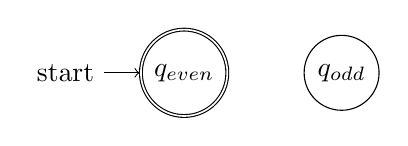
\begin{tikzpicture}[auto, node distance=2cm]
        \node[initial,state,accepting] (even) {\(q_{even}\)};
        \node[state] (odd) [right of=even] {\(q_{odd}\)};
    \end{tikzpicture}
    \pause
    \item Labelled arrows between states for transitions (next state logic) \\
    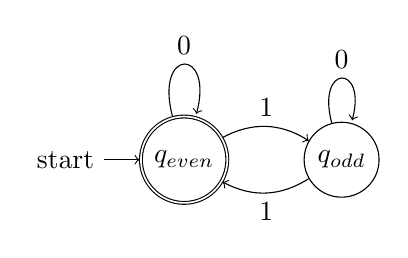
\begin{tikzpicture}[auto, node distance=2cm]
    \centering
        \node[initial,state,accepting] (even) {\(q_{even}\)};
        \node[state] (odd) [right of=even] {\(q_{odd}\)};
        \path[->](even) edge [loop above] node {0} (even);
        \path[->](even) edge [bend left] node {1} (odd);
        \path[->] (odd) edge [loop above] node {0} (odd);
        \path[->] (odd) edge [bend left] node {1} (even);
    \end{tikzpicture}
\end{itemize}
\end{frame}
\begin{frame}{Languages}
\begin{itemize}
    \item A \emph{Language} over an alphabet is a subset of \(\Sigma^*\).
    \item The output of a DFA is either accept or reject - correspondingly, we can define the \emph{language recognised by a DFA} by including all strings it accepts and excluding strings it rejects. Call this the \emph{language of a DFA}.
    \item This works for decision problems - If the \( \mathcal{O} \) has three elements instead of two, we cannot directly define the language of the machine.
\end{itemize}
\end{frame}
\begin{frame}{Some Simple DFAs}
    \begin{itemize}
        \item Does \texttt{0010} appear in a bitstring?
        \item Is the number of \texttt{0}s in a bitstring divisible by 7?
        \item Is a decimal number even?
        \item Is a decimal number divisible by 3, 5, 9, 10, 1000, 250000000? \(2^{100}\)?
        \item Is a decimal number divisible by 45, 225 or  4500?
        \item Dvisibility by any constant, actually.
        \item Is there a 3-tuple \(a = a_1a_2a_3 \in \Sigma^3\) such that the input is of the form \(a^n = a\circ a \circ a \dots\)? What is \(|Q |\)?
        \item Is the input ``\texttt{washing powder nirma}''?
        \item Is the input an element of $\langle$\emph{insert finite set}$\rangle$? Is it a Martin Luther King speech?
        \item Is the length of the input \(2^n\) for some \( n \in \{1, 2, 3, \dots 100, 105, 53770\}\)?
    \end{itemize}
\end{frame}
\begin{frame}{Analysis of a DFA}
\begin{itemize}
    \item Looks at an character in the string only once.
    \item The state is a \emph{summary} of the part of the string encountered until that point.
    \item Does not ``know'' how many elements in the stream have been seen! The ``summary'' can count only till a finite number as \( |Q| \) is finite. There is no bound on the length of input strings.\pause
    \item Fact: There exist languages (obviously infinite) that a DFA cannot \emph{recognise}.\pause
\end{itemize}    
\end{frame}
\begin{frame}{Problems a DFA cannot compute}
\begin{itemize}
    \item Is the number of \texttt{0}s more than the number of \texttt{1}s?
    \item More generally, which character has the highest, lowest or third highest frequency?
    \item Is the input a prime number?
    \item Is the length of the input of the form \(2^n\)?
    \item Graph Isomorphism? (Check yourself)
\end{itemize}
\end{frame}
\begin{frame}{Why finite automata?}
\begin{block} {What happens if we allow \(Q\) to be an infinite set?}\pause
\begin{itemize}
    \item The DFA can store the entire input!\pause
    \item \( \delta\) has an infinite domain - can we implement it? (Although we don't care.)
    \item Embed a 'normal' computer in the next-state logic and compute the output?
    \item Use an infinite lookup table?
\end{itemize}
\end{block}
\pause
The power (and realisability) of automata changes dramatically if we permit \(Q\) to be infinite.\\
Hard-coding the language in the transition function is the simplest strategy we can use.
\end{frame}
\begin{frame}{Computability}
    \begin{block}{Regular Languages}
        A language is regular if there exists a deterministic finite automaton recognising it.
    \end{block}
    \pause
    \begin{alertblock}{Power of DFAs}
        There exist languages that can be recognised by certain models of computation (like general-purpose computers) but not DFAs.
    \end{alertblock}
    \pause
    \begin{alertblock}{Decidability}
        There exist languages that cannot be recognised by any realisable model of computation. (Called undecidable languages.)
    \end{alertblock}
\end{frame}
\begin{frame}{Complexity Considerations}\pause
\begin{itemize}
    \item Need at least \(c\cdot n \) units of time to \emph{look} at the input, whose length is \(n\). (Holds for any model of computation.) \pause
    \item Define \( \delta_t : Q \times \Sigma \rightarrow \mathbb{R}, \delta_t(q, a)\) is the time needed to compute \(\delta(q, a)\) and make the transition. Then, clearly, there is a minimum $t_{min}$ and a maximum $t_{max}$ value in the range of the function - there are finitely many transitions possible. \pause
    \item We obtain upper and lower bounds on the time $t_s$ needed to compute the output on a string $s$ of length $ |s|$: \[t_s \in [|s|t_{min}, |s|t_{max}] \]. Linear in the length of the input - \emph{optimal} value. \pause
    \item \alert{Time Complexity} is not a thing here. (Not so for infinite automata.)
\end{itemize}
\end{frame}
\begin{frame}{Complexity Considerations}
Computing the transition function may need a complex mechanism if \( |\Sigma |\) or \(|Q|\) is large. Large alphabets and and state spaces roughly correspond to increasing the data encoded in the input and the memory of the machine, respectively.
\begin{itemize}
\item For a given alphabet, we can rewrite each string by replacing each character with a bitstring of length \( \log_2 |\Sigma |\) and replacing \(Q\text{ by } Q \times \{0, 1, * \}^{ \lceil \log_2 |\Sigma | - 1 \rceil}\), so that the ``summary'' of the input until that point is effectively the summary of the original alphabet until the last block and the bits in the current block.
\item There are minor changes in the transition function - it interprets bitstrings as characters of the original alphabet on reaching the end of each block.
\item These changes produce a constant increase in the complexity of the machine and its functioning, and are not of interest in TCS.
\end{itemize}
\end{frame}
\begin{frame}{Nondeterminism}
\pause
\begin{itemize}
    \item Deterministic computation - Next state is a function of current state of the system, no ambiguity.
    \pause
    \item Nondeterministic computation - Next state depends on current state, but there isn't a simple 'next state' - there may be multiple or none.
    \pause
    \item Parallel computation in some sense. You can imagine \emph{clones} of the machine being created. There is branching.
    \pause
    \item Input is accepted if one of the branches is at an accept state at the end.
    \pause
    \item It is a theoretical construct. Physical systems are deterministic.
\end{itemize}
    [ \href{https://www3.cs.stonybrook.edu/~cse350/slides/automata5.pdf}{Detailed Explanation} ]
\end{frame}
\begin{frame}{Nondeterminism}
\includegraphics[scale=0.9]{automata/nondeterminism.png}    
    \href{https://www3.cs.stonybrook.edu/~cse350/slides/automata5.pdf}{Source}
\end{frame}
\begin{frame}{Technicalities}
We include the empty string \( \varepsilon\) in the alphabet.
\begin{block}{Nondeterministic Finite Automaton}
A nondeterministic finite automaton is a 5-tuple \( (Q, \Sigma, \delta, q_0, F) \) where
    \begin{enumerate}
        \item \(Q\) is a finite set of states.
        \item \(\Sigma\) is an alphabet
        \item \(\delta: \Sigma_\varepsilon \times Q \rightarrow \mathcal{P}(Q)\) is the transition function, where \(\Sigma_\varepsilon = \Sigma \cup \{\varepsilon\}\), \(\mathcal{P}(\cdot)\) is the power set - set of all subsets
        \item \(q_0 \in Q\) is the initial state
        \item \( F \subseteq Q\) is the set of accept states.
    \end{enumerate}
    \end{block}
The difference is in the transition function - the machine can go to multiple states or no state instead of only one.\\
Each branch resides in a state. Together, the clones, define a \emph{subset} of \(Q\).
\end{frame}
\begin{frame}{Schematic}
\includegraphics[scale=1]{automata/nfa_graph.png}
\begin{itemize}
    \item Multiple arrows exiting a state with the same label - instances of branching.
    \item In some cases, there is no arrow with a particular label. In that case, that branch of the computation 'dies' and we can ignore it. (Fancy way to enter a reject state.)
    \item If \(\delta( \varepsilon, r_i)\) is a nonempty set, the machine enters all the states in the set without reading the next character. A copy of the machine remains in the state \(r_i\).
\end{itemize}
\end{frame}
\begin{frame}{Accepting and Rejecting Inputs}
\begin{block}{Operation of an NFA}
    A NFA \(N = (Q, \Sigma, \delta, q_0, F) \) accepts a string \(y = y_1y_2y_3\dots y_m\) if there exists a sequence of states (a branch of computation) \(r_0 r_1 r_2 \dots r_m \in Q^{m+1}\) with \begin{enumerate}
        \item \(r_0 = q_0\) (Initially in the start state)
        \item \(r_{i+1} \in \delta (y_{i+1}, r_i)\)
        \item \(r_m \in F\)
    \end{enumerate}
\end{block}
\pause
The condition for accepting a string can be redefined in terms of the set of states the machine is in at level \(i\) in the computation.
\end{frame}
\begin{frame}{NFAs}
The set of states is a subset of \(Q\), so it is an element of another finite set. (Like a DFA!)\\
\includegraphics[scale=0.5]{automata/nfa_tree.png}
\end{frame}
\begin{frame}{Equivalence of DFAs and NFAs}
\begin{block}{Theorem}
Every NFA \(N= (Q, \Sigma, \delta, q_0, F)\) has a DFA \( D_N = (Q', \Sigma, \delta', q_0, F') \) that recognises the same language.
\begin{itemize}
    \item \(Q' := \mathcal{P}(Q)\)
    \item \(\delta' (R, a) := \bigcup_{r \in R} \delta (r, a)\)
    \item \(F' := \{ A \subseteq Q | A \text{ contains an accept state, ie } A \cap F \neq \phi \} \)
\end{itemize}
\end{block}
    We call two automata \emph{equivalent} if they recognise the same language.
    \pause
\begin{alertblock}{Summary}
    Nondeterminism does not make a DFA more \emph{powerful}! \\ \pause
    Broadly speaking, this is because a DFA has finite memory. \\\pause However, \emph{pushdown} automata are more powerful than DFAs. Nondeterministic pushdown automata are even more powerful.
\end{alertblock}
\end{frame}
\begin{frame}{Certificates and Nondeterminism}
Suppose a language \(\mathcal{L}\) is defined by a property \(\mathtt{P}\), and we use a NFA to test strings for \(\mathtt{P}\).\pause
\begin{itemize}
    \item Using a DFA isn't always practical because the state space \(Q'\) has exponential size.
    \item Supposing the property holds for \(y=y_1 y_2 y_3 \dots y_m\), then a imaginary NFA could output the sequence of states \(r_0 r_1 r_2 \dots r_m\) and we can verify that each transition is valid in the sequence, ie that the sequence was indeed the path taken in the tree by one of the clones. In reasonable time!
    \item This is called a certificate - a reasonable-sized (about as long as the input), reasonable-time verifiable string or piece of data that testifies to a property of the input.
    \item Nondeterministic computation is related to certificates of membership or non-membership.
\end{itemize}
\end{frame}
\begin{frame}{Examples of Certificates}
    \begin{itemize}
        \item Graph isomorphism - the bijection is a certificate
        \item Group isomorphism - the bijection
        \item Composite numbers - output a factor
        \item \emph{Satisfiability} of boolean formulas - output the satisfying assignment (or row in the truth table)
        \item Non-union closed families of sets
        \item Reachability and distance in a graph - can you travel between two vertices in \( \leq k\) steps?
    \end{itemize}
Will discuss further in Turing Machines.\\
Some cryptography protocols use difficult-to-find certificates, that adversaries can't reverse-engineer.
\end{frame}
\end{document}

